\chapter{Abläufe}

\section{Sequenzdiagramme}

\subsection{Ende einer Challenge}

Der in der Challenge vom Spieler bearbeitete Knoten vom Typ \class{Knot} ruft bei Kantenänderungen durch den Spieler eine Methode auf, die ihm beim Hinzufügen zum \class{ChallengeModeScreen} zugewiesen wurde. Diese prüft die beiden Knoten auf Gleichheit, indem sie die Knoten sich über die Methode Equals(Knot) vergleichen lässt. Sind beide \class{Knot}en gleich, wird die benötigte Zeit ermittelt und ein neuer \class{Dialog} erstellt, der die Zeit anzeigt und nach einem Benutzernamen fragt.
\newline
\newline
Dazu wird aus Options.Default der Benutzernamen abgefragt und als Standardwert eingetragen. Wird ein neuer Benutzername eingegeben, wird dieser auch in Options.Default geändert. Mit Enter bestätigt wird eine zugewiesene Methode aufgerufen, die Benutzername und Zeit dem \class{Challenge}-Objekt mit AddToHighscore(name, time) übergibt, was die Werte richtig einordnet und gegebenenfalls (wenn die Zeit gut genug ist) speichert.
\newline
\newline
Daraufhin öffnet diese Methode einen neuen \class{Dialog}, der, soweit vorhanden, die besten zehn Einträge sowie zwei Buttons anzeigt, von denen einer die \class{Challenge} neu startet und ein anderer den \class{StartScreen} aufruft. Obwohl nur die besten zehn Highscore-Einträge angezeigt werden, sind trotzdem alle bisher hinzugefügten Einträge sowohl in dem Challenge-Objekt als auch in dem Speicherformat der Challenge enthalten, da sie zur Berechnung der durchschnittlichen Zeit benötigt werden, die u.A. im \class{ChallengeStartScreen} zu jeder Challenge angezeigt werden kann.

\subsection{Screenwechsel von dem CreativeMainScreen in den CreativeLoadScreen}

Wenn man in dem Menü, das durch den \class{CreativeMainScreen} dargestellt wird, auf den Button "Load" klickt, wird der Wechsel zu \class{CreativeLoadScreen} eingeleitet. Dabei wird ein neues \class{CreativeLoadScreen} erstellt und oben auf den Stack in \class{Knot3Game} gelegt, in dem die Spielstände abgespeichert werden.
\newline
\newline
Beim nächsten Update()-Call des XNA-Frameworks wird der PostProcessingEffect von \class{CreativeLoadScreen} für ein Überblenden der Rendertargets auf \class{FadeEffect} gesetzt und der \class{CreativeMainScreen} wird deaktiviert, d.h. alle \interface{IGameScreenComponent}s von \class{CreativeMainScreen} werden aus der Liste der aktuell in XNA registrierten \interface{IGameScreenComponent} gelöscht. Außerdem wird die BeforeExit()-Methode von \class{CreativeMainScreen} aufgerufen, in der eventuell anfallende Aufräumarbeiten ausgeführt werden können.
\newline
\newline
Dann wird \class{CreativeLoadScreen} aktiviert und dessen Entered()-Methode aufgerufen, die dessen \interface{IGameScreenComponent}s mittels der in \class{GameScreen} implementierten AddGameComponents()-Methode in die \xna{IGameComponent}-Liste des XNA-Frameworks einträgt. Diese Operation ist rekursiv, d.h. die über die SubComponents()-Methode jedes \interface{IGameScreenComponent}s ermittelten Unterkomponenten werden von AddGameComponents() ebenfalls erfasst.
\newline
\newline
In diesem Beispiel wäre eine direkt von \class{CreativeLoadScreen} hinzugefügte Komponente das Spielstand-Menü, das von der Klasse \class{VerticalMenu} repräsentiert wird. Dieses gibt über die SubComponents()-Methode alle in dem Menü enthaltenen \class{MenuItem}s zurück, damit diese von AddGameComponents() ebenfalls als \interface{IGameScreenComponent} registriert und dargestellt werden können.
\newline
\newline
Daraufhin durchsucht \class{CreativeLoadScreen} das Spielstand-Verzeichnis und lädt die Metadaten der Speicherstände aller zwischengespeicherten Knoten.
Noch nicht zwischengespeicherte Knoten werden auf Gültigkeit überprüft und wenn für Gültig befunden in den Zwischenspeicher geschrieben als Hash.
\newline
\newline
Anschließend werden die gefundenen gültigen Spielstände in ein Menü eingetragen, welches dann beim nächsten Draw()-Call von XNA auf den Bildschirm gezeichnet wird.
Dieses Menü ist ein \class{VerticalMenu}, welches einen \class{MenuButton} für jeden gültigen gefundenen Spielstand enthält. Durch einen Klick auf den jeweiligen Button startet man mit dem Spielstand im \class{CreativeModeScreen}.

\subsection{Erstellen der 3D-Objekte nach durchgeführten Kantenverschiebungen}

Sowohl im \class{CreativeModeScreen} als auch im \class{ChallengeModeScreen} wird ein \class{Knot}en vom Spieler bearbeitet, auf Basis dessen mittels einer Instanz von \class{KnotRenderer} 3D-Modell-Objekte, die von \class{GameModel} und \interface{IGameObject} erben, erstellt werden. Dazu wird die OnEdgesChanged()-Methode der \class{KnotRenderer}-Klasse dem EdgesChanged()-Delegate des \class{Knot}-Objekts zugewiesen, sodass der \class{KnotRenderer} bei allen Kantenänderungen benachrichtigt wird.
\newline
\newline
Wurde eine Kantenänderung durchgeführt und OnEdgesChanged() auf dem \class{KnotRenderer} aufgerufen, so leert dieser zunächst seine drei Listen mit den bisher vorhandenen \class{PipeModel}s (als Röhren dargestellte Kanten), \class{NodeModel}s (Übergänge zwischen zwei Kanten) und \class{ArrowModel}s (Pfeile an selektierten Kanten).
\newline
\newline
Nun ruft der \class{KnotRenderer} die OnEdgesChanged()-Methode auf einem von ihm gehaltenen \class{NodeMap}-Objekt auf, um für alle Kanten des \class{Knot}s eine Zuordnung zwischen dem \class{Edge}-Objekt und der jeweiligen Position im 3D-Raster zu erstellen, welche von \class{Node} repräsentiert wird. Ein Objekt der Klasse \class{Node} hält dabei einen Rasterpunkt, wobei der Abstand zwischen den zwei \class{Node}s, an denen eine Kanten beginnt und endet, den normalisierten Abstand $1$ hat. Die Konvertierung in 3D-Koordinaten in Form von Vector3-Objekten erfolgt später in den über die ToVector()-Methode der \class{Node}-Objekte.
\newline
\newline
Daraufhin werden für alle drei Kategorien neue Modell-Informationen erstellt, welche von Objekten der Klassen \class{PipeModelInfo}, \class{NodeModelInfo} und \class{ArrowModelInfo} repräsentiert werden. Dabei wird jeweils ein als Attribut der Klasse \class{KnotRenderer} vorhandenes \class{ModelFactory}-Objekt verwendet, um bereits vor der Verschiebeaktion vorhandene Modell-Objekte wiederzuverwenden und nur bisher nicht vorhandene Modell-Objekte neu zu erstellen. Die Klasse \class{ModelFactory} implementiert dabei einen Cache, der über eine Hashtabelle beliebige \class{GameModelInfo}-Objekte daraus generierten \class{GameModel}-Objekten zuordnet. Die Erstellung neuer Objekte erfolgt dabei durch ein Delegate, das bei der Erstellung einer \class{ModelFactory} ihrem Konstruktor übergeben wird.
\newline
\newline
Die Erstellung der Modell-Objekte erfolgt wie nachfolgend beschrieben.

\subsection{Verschiebung einer Kante}
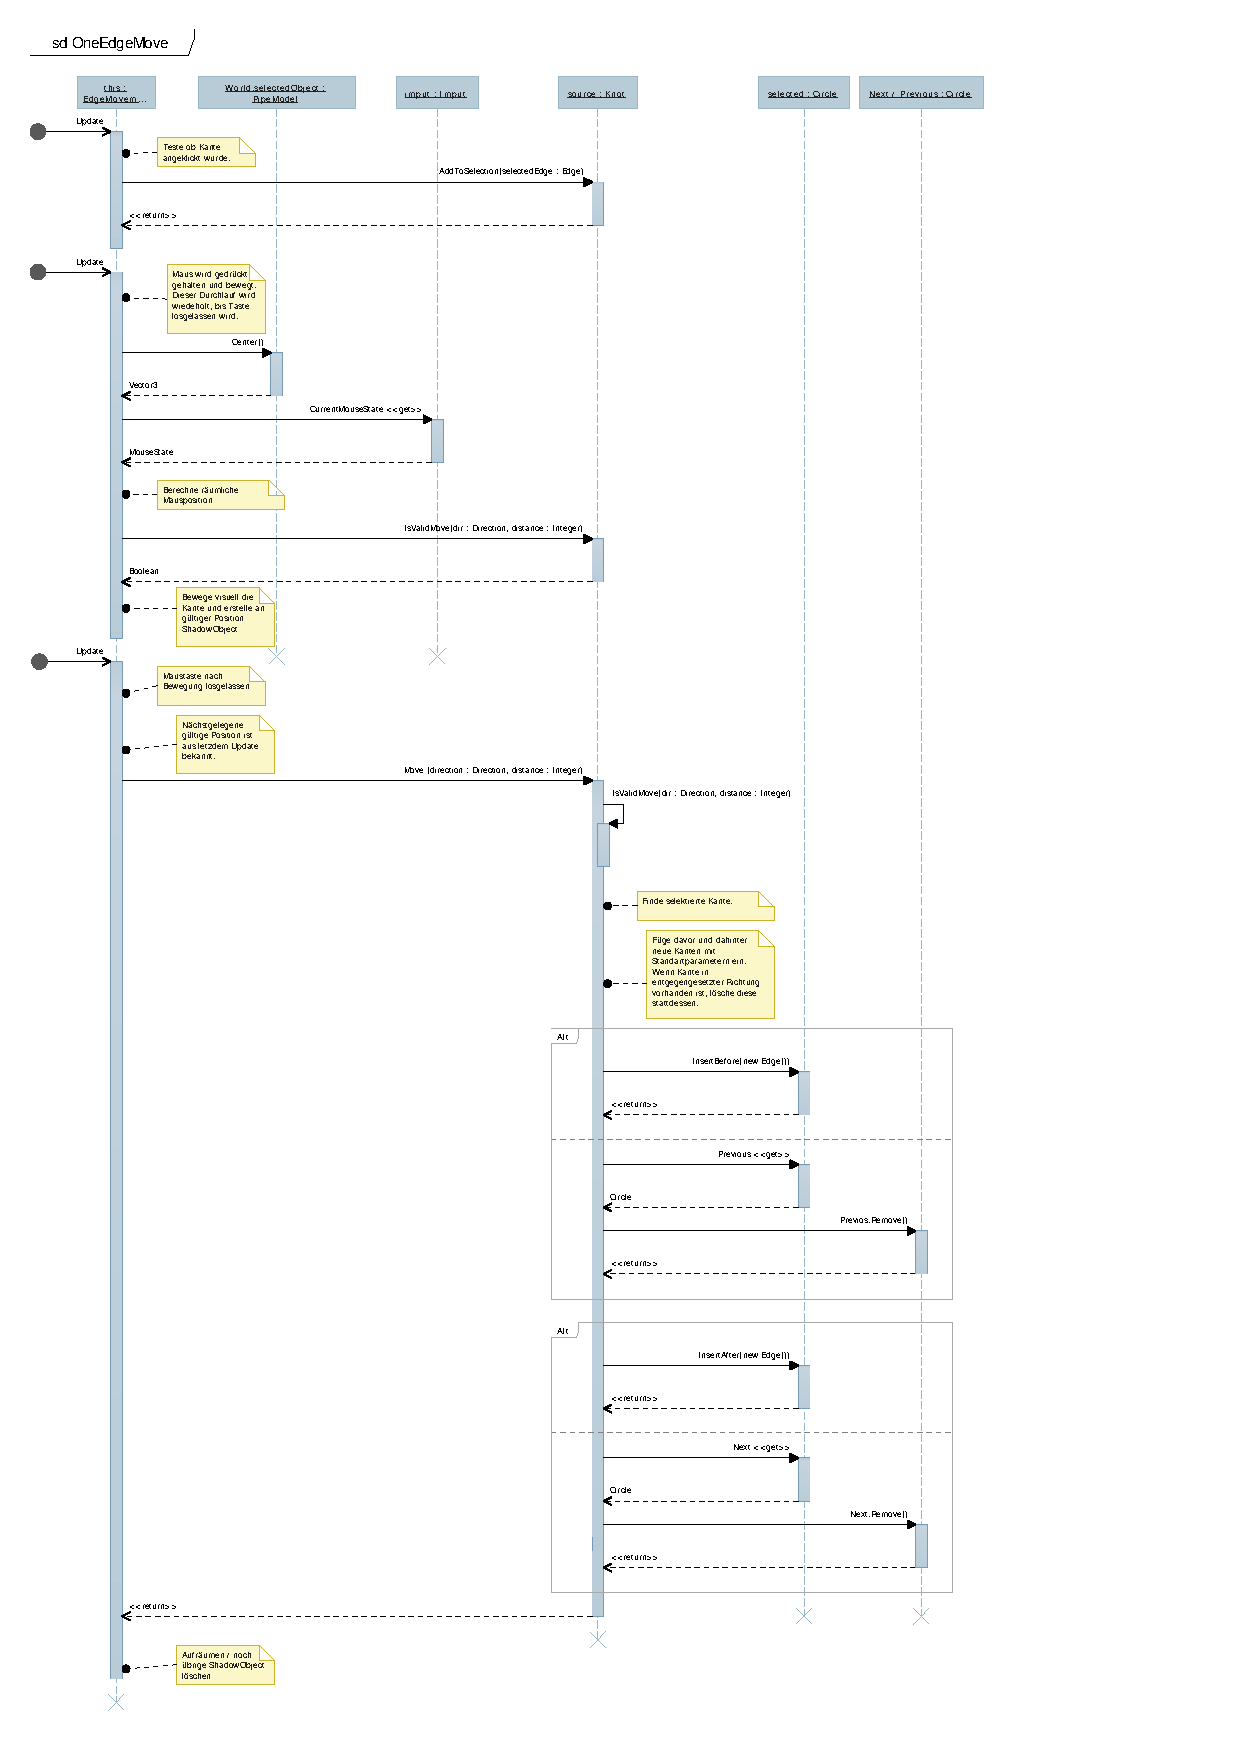
\includegraphics[scale=0.8]{Sequenzdiagram_OnEdgeMove.pdf}

\paragraph{Kanten}

Um für alle aktuell im \class{Knot}en vorhandenen Kanten eine jeweils Röhre (\class{PipeModel}) zu erstellen, wird über die im \class{Knot}-Objekt enthaltenen \class{Edge}-Objekte iteriert. Für jede \class{Edge} wird ein \class{PipeModelInfo} erstellt, dem im Konstruktor der \class{Knot}en, die \class{Edge} sowie die \class{NodeMap} übergeben werden. Die \class{PipeModelInfo}-Instanz berechnet daraus dann die Position der Röhre sowie weitere zur Darstellung notwendige Daten. Mit Hilfe dieser Modellinformationen werden dann jeweils über die zuständige \class{ModelFactory} die bereits vorhandenen \class{PipeModel}-Objekte abgefragt bzw. neu erstellt und der \class{PipeModel}-Liste des \class{KnotRenderer}s zugewiesen.

\paragraph{Kantenübergänge}

Da die 3D-Modelle, die an den Kantenübergängen dargestellt werden, sich abhängig von der Anzahl der an dem Rasterpunkt angrenzenden Kanten und ihrer Positionen unterscheiden, wird für die Bestimmung der 3D-Modelle zunächst eine Zuordnung zwischen den Rasterpunkten (\class{Node}) und einer Liste von einzelnen Kantenübergängen (\class{IJunction}) durch Iteration über die \class{Edge}s bzw. den zugehörigen \class{Node}s erstellt. Das Interface IJunction enthält Informationen über die eingehende und ausgehende \class{Edge} und wird von der Klasse \class{NodeModelInfo} implementiert, die im Konstruktur diese beiden Objekte sowie eine Referenz auf die \class{NodeMap} erwartet.
\newline\newline
Danach wird für alle Rasterpunkte entschieden, wie viele und welche 3D-Modelle zur Darstellung des Kantenübergangs benötigt werden. Dabei werden zwischen null und drei \class{NodeModelInfo}-Objekte mit teilweise unterschiedlichen Modell-Dateien, Drehungen und Skalierungen erstellt, aus denen mit Hilfe der für \class{NodeModel}-Objekte zuständigen \class{ModelFactory}-Instanz die entsprechenden \class{NodeModel}-Objekte abgefragt bzw. erstellt werden. Diese werden dann, analog zu dem Vorgehen bei den \class{PipeModel}-Objekten, in die \class{NodeModel}-Liste des \class{KnotRenderer}s eingefügt.

\paragraph{Pfeile}

Zur Erstellung der Modellinformationen der \class{ArrowModel}s wird zunächst über die Liste der selektierten Kanten iteriert, um die Kante zu finden, die sich in der Mitte der selektierten Kantenfolge befindet. An dieser Position soll, unter Umständen um einen noch zu bestimmenden Abstand in Richtung der Kameraposition verschoben, für jede gültige Richtung, in welche die selektierten Kanten verschoben werden können, ein Pfeil angezeigt werden. Dabei wird die Distanz der Verschiebung nicht in der Berechnung berücksichtigt; es reicht aus, wenn mindestens eine Distanz existiert, in die dieser Zug gültig wäre.
\newline\newline
Für die ermittelten gültigen Pfeilrichtungen wird jeweils ein \class{ArrowModelInfo}-Objekt erstellt, das zur Abfrage und Erstellung von \class{ArrowModel}-Objekten über die zugehörige \class{ModelFactory} verwendet wird. Die erstellten \class{ArrowModel}-Objekte werden in die \class{ArrowModel}-Liste des \class{KnotRenderer}s eingefügt. Falls keine Kanten selektiert sind, ist die Liste der Pfeilmodelle leer.
\newline\newline
Dieses Erstellen von \class{ArrowModel}-Objekten bei einer Selektion von Kanten kann in den Einstellungen des Spiels über eine Option deaktiviert werden. In diesem Fall werden Verschiebeoperationen nur direkt durch Anklicken und Ziehen an den Kanten ausgeführt; diese Möglichkeit ist dem Spieler auch gegeben, wenn die Pfeil-Anzeige aktiviert ist.
\newline\newline
Damit die \class{ArrowModel}-Objekte nicht nur nach Verschiebe-Aktionen, sondern auch nach einer Änderung der Kantenauswahl mit dem beschriebenen Algorithmus neu erstellt werden, wird der pfeilbezogene Teil des beschriebenen Algorithmus in eine private Methode ausgelagert. Diese wird einierseits nach dem Erstellen der \class{PipeModel}- und \class{NodeModel}-Objekte über die OnEdgesChanged()-Methode aufgerufen, andererseits wird sie bei der Zuweisung eines \class{Knot}ens zur aktuellen \class{KnotRenderer}-Instanz auch in das SelectionChanged()-Delegate des \class{Knot}en eingefügt, um ebenfalls bei allen Auswahländerungen benachrichtigt zu werden.

